\section{条件重建与比较协议}
\label{sec:supp-protocol}
主比较评价给定相机及参与者状态下的重建，最后四帧评价条件时间外推。表~\ref{tab:shared-inputs} 列出测试条件。目标人体关节来自独立离线标注／拟合，人体体型和绑定由上下文恢复，测试 LiDAR 专用于评价。测试时全部网络权重固定。

\paragraph{训练资源。}
STORM、DGGT 和 StreetForward 保留各自原生结构，随机初始化重训。每种方法使用相同真实训练日志 $D_R$、合成场景 $D_S$ 和完整资产 $D_A$。基线通过自身目标接收 RGB、深度、轮廓及完整资产目标视图监督，Ours 另用单元空域和模板绑定监督。各方法在固定预算内训练，并在共同开发集上选择 checkpoint（表~\ref{tab:baseline-resources}）。CCM 消融匹配恢复模块、codec、数据和优化预算，以测量组件交换的贡献。

\begin{table*}[t]
\centering\small
\caption{单个完整 checkpoint 的训练资源，包含方法专用目标预处理。Ours 和 w/o CCM 均计入共享恢复模块与 codec 的成本。}
\label{tab:baseline-resources}
\begin{tabular}{@{}lp{0.39\textwidth}rrr@{}}
\toprule
方法 & 训练目标 & 更新步数 & 全局 batch & GPU 小时 \\
\midrule
STORM & 原生重建及同源合成视图 & 234,816 & 16 & 916.7 \\
DGGT & 原生几何／渲染及同源合成视图 & 212,672 & 16 & 1,128.4 \\
StreetForward & 原生场景重建及同源合成视图 & 246,144 & 8 & 1,036.9 \\
Ours & 完整四阶段 & 287,360 & 分阶段 & 1,001.5 \\
w/o CCM & 共享 R/C，重训 GCM 先验及适配 & 287,360 & 同 Ours & 977.1 \\
\bottomrule
\end{tabular}
\end{table*}

\paragraph{统一状态适配器。}
各基线使用共同的确定性状态适配器。将高斯可见渲染贡献投到同一组上下文实例掩码，累积加权身份票。车辆依据给定根位姿执行逆 SE(3)，同时变换中心、协方差和方向坐标基。人体高斯在上下文恢复的同身份模板上匹配三角形，以重心插值得到 17 关节蒙皮权重，再执行逆蒙皮。适配器保留预测外观，不增加预测网络。未绑定输出保留评价，无法装配的参与者编辑计为失败。

同一高斯集合经逆变换和正变换后，最大线性 RGB 差低于 $4\times10^{-6}$。将原生时变表示转换为固定规范资产的跨时刻重建变化见表~\ref{tab:adapter-effect}，适配后列用于正文主比较。

\begin{table}[t]
\centering\small
\caption{转为固定规范资产对重建的影响，PSNR 单位为 dB。}
\label{tab:adapter-effect}
\begin{tabular}{@{}lrrr@{}}
\toprule
方法 & 原生 & 适配后 & 差值 \\
\midrule
STORM & 26.492 & 26.380 & $-0.112$ \\
DGGT & 27.538 & 27.410 & $-0.128$ \\
StreetForward & 27.094 & 27.010 & $-0.084$ \\
\bottomrule
\end{tabular}
\end{table}

\begin{table*}[!t]
\centering\small
\setlength{\tabcolsep}{4pt}
\caption{DriveCompose、STORM、DGGT 和 StreetForward 的共同测试条件。}
\label{tab:shared-inputs}
\begin{tabular}{@{}lp{0.67\textwidth}@{}}
\toprule
条件 & 统一设置 \\
\midrule
上下文 RGB & 相同四时刻、三相机 \\
相机与自车状态 & 统一给定内外参及自车位姿 \\
测试深度/LiDAR & 不作为输入；深度由 RGB 估计 \\
身份、车辆框与根轨迹 & 统一给定 \\
人体体型与绑定 & 上下文恢复，统一绑定接口 \\
目标人体关节 & 独立离线标注/拟合，统一给定 \\
测试场景优化 & 全部关闭 \\
\bottomrule
\end{tabular}
\end{table*}

每条测试序列取前 200 个有效同步帧，形成 10 个不重叠的 20 帧片段，共 2,020 个片段。三相机上下文索引为 $\{0,5,10,15\}$，其余 12 帧插值产生 72,720 张图像，$\{16,17,18,19\}$ 四帧外推产生 24,240 张图像，共 96,960 张。全部目标时刻具有有效动态掩码和深度评价样本。表~\ref{tab:temporal-groups} 按插值／外推 $3{:}1$ 汇总，恢复主表均值。深度尺度对齐仅用于评价，不反馈给重建或渲染。

\begin{table*}[!t]
\centering\small
\setlength{\tabcolsep}{4pt}
\caption{时间插值与条件外推。全图和动态区域为 PSNR/SSIM，深度为逐帧尺度对齐的 AbsRel/$\delta_1$。}
\label{tab:temporal-groups}
\begin{tabular}{@{}lcccc@{}}
\toprule
方法 & 时间组 & 全图 & 动态区域 & 深度 \\
\midrule
STORM & 插值 & 26.800/0.838 & 22.600/0.640 & 0.170/0.753 \\
STORM & 外推 & 25.120/0.790 & 20.600/0.576 & 0.202/0.705 \\
DGGT & 插值 & 27.800/0.806 & 23.200/0.667 & 0.237/0.680 \\
DGGT & 外推 & 26.240/0.758 & 21.240/0.603 & 0.285/0.632 \\
StreetForward & 插值 & 27.400/0.830 & 21.500/0.608 & 0.185/0.771 \\
StreetForward & 外推 & 25.840/0.782 & 19.176/0.544 & 0.233/0.723 \\
Ours & 插值 & \textbf{28.900/0.909} & \textbf{25.500/0.870} & \textbf{0.091/0.885} \\
Ours & 外推 & \textbf{27.556/0.877} & \textbf{23.700/0.838} & \textbf{0.107/0.853} \\
\bottomrule
\end{tabular}
\end{table*}

\paragraph{深度尺度与米制评价。}
对齐深度列在固定有效 LiDAR 掩码 $M_t$ 上估计逐帧正尺度：
\begin{equation}
s_t=\operatorname{median}_{p\in M_t}\frac{d_t(p)}{\widehat d_t(p)}.
\label{eq:depth-alignment}
\end{equation}
拟合量为单一尺度。表~\ref{tab:depth-scale} 的对齐与未对齐深度使用相同掩码，按帧、片段和序列依次汇总。尺度对齐在深度评价器内执行；重建、装配、表面距离和 RGB 重投影使用原始米制坐标。

\begin{table*}[t]
\centering\small
\caption{逐帧尺度对齐与未对齐深度评价。}
\label{tab:depth-scale}
\begin{tabular}{@{}lrrrr@{}}
\toprule
& \multicolumn{2}{c}{逐帧尺度对齐} & \multicolumn{2}{c}{未对齐} \\
\cmidrule(lr){2-3}\cmidrule(lr){4-5}
方法 & AbsRel $\downarrow$ & $\delta_1\uparrow$ & AbsRel $\downarrow$ & $\delta_1\uparrow$ \\
\midrule
STORM & 0.178 & 0.741 & 0.226 & 0.683 \\
DGGT & 0.249 & 0.668 & 0.327 & 0.572 \\
StreetForward & 0.197 & 0.759 & 0.254 & 0.694 \\
Ours & \textbf{0.095} & \textbf{0.877} & \textbf{0.121} & \textbf{0.842} \\
\bottomrule
\end{tabular}
\end{table*}

\section{消融、种子统计与评价分母}
\label{sec:supp-ablations}
两个学习版本使用训练种子 $\{0,1,2\}$，每个 checkpoint 评价生成种子 $\{7,17,27\}$，形成九组结果。先平均生成种子，再按帧、窗口、序列及训练种子等权汇总，不采用 best-of-three。表~\ref{tab:seed-components} 和表~\ref{tab:seed-inputs} 每格为均值 $\pm$ 三个训练种子均值的样本 SD，括号内为生成种子的平均样本 SD。w/o GCM 的零波动对应固定共享恢复模块和 codec 后的确定性推理。

\begin{table*}[!t]
\centering\small
\setlength{\tabcolsep}{4pt}
\caption{组件消融的完整种子统计。}
\label{tab:seed-components}
\begin{tabular}{@{}lccc@{}}
\toprule
指标 & w/o GCM & w/o CCM & Ours \\
\midrule
全图 PSNR & 27.137 $\pm$ 0 & 28.286 $\pm$ 0.074 (0.032) & \textbf{28.913 $\pm$ 0.061 (0.028)} \\
全图 SSIM & 0.867 $\pm$ 0 & 0.893 $\pm$ 0.001 (0.0006) & \textbf{0.911 $\pm$ 0.001 (0.0005)} \\
全图 LPIPS & 0.183 $\pm$ 0 & 0.147 $\pm$ 0.002 (0.0013) & \textbf{0.129 $\pm$ 0.002 (0.0011)} \\
动态 PSNR & 23.431 $\pm$ 0 & 24.683 $\pm$ 0.112 (0.048) & \textbf{25.617 $\pm$ 0.095 (0.041)} \\
动态 SSIM & 0.811 $\pm$ 0 & 0.849 $\pm$ 0.002 (0.0010) & \textbf{0.873 $\pm$ 0.002 (0.0008)} \\
\bottomrule
\end{tabular}
\end{table*}

\begin{table*}[!t]
\centering\small
\setlength{\tabcolsep}{4pt}
\caption{固定权重的输入时刻数量敏感性；$T=8$ 复用组件表结果。}
\label{tab:seed-inputs}
\begin{tabular}{@{}lcccc@{}}
\toprule
$T$ & 版本 & PSNR $\uparrow$ & SSIM $\uparrow$ & LPIPS $\downarrow$ \\
\midrule
2 & w/o CCM & 25.237 $\pm$ 0.103 (0.055) & 0.817 $\pm$ 0.003 (0.0011) & 0.254 $\pm$ 0.004 (0.0023) \\
2 & Ours & \textbf{26.341 $\pm$ 0.089 (0.047)} & \textbf{0.851 $\pm$ 0.002 (0.0009)} & \textbf{0.213 $\pm$ 0.003 (0.0019)} \\
4 & w/o CCM & 27.126 $\pm$ 0.086 (0.041) & 0.869 $\pm$ 0.002 (0.0008) & 0.187 $\pm$ 0.003 (0.0018) \\
4 & Ours & \textbf{27.864 $\pm$ 0.072 (0.035)} & \textbf{0.891 $\pm$ 0.001 (0.0006)} & \textbf{0.159 $\pm$ 0.002 (0.0014)} \\
8 & w/o CCM & 28.286 $\pm$ 0.074 (0.032) & 0.893 $\pm$ 0.001 (0.0006) & 0.147 $\pm$ 0.002 (0.0013) \\
8 & Ours & \textbf{28.913 $\pm$ 0.061 (0.028)} & \textbf{0.911 $\pm$ 0.001 (0.0005)} & \textbf{0.129 $\pm$ 0.002 (0.0011)} \\
\bottomrule
\end{tabular}
\end{table*}

每条测试序列取一个 29 时刻窗口，共 202 个。$\mathcal T_2=\{0,28\}$、$\mathcal T_4=\{0,8,20,28\}$、$\mathcal T_8=\{0,4,\ldots,28\}$ 共享 $\{2,6,\ldots,26\}$ 七个目标时刻及三相机，每组共 4,242 张目标图像。两个学习版本、三个 $T$、九个种子组合共 54 组、229,068 张预测图像。w/o GCM 另有 4,242 张，总计 233,310 张。

不可渲染数为学习版本 $0/10,908$ 个窗口实例、w/o GCM $0/202$。低质量、空洞和接触错误均保留计分。所有变体共享图像预处理、$240\times160$ 分辨率、标注动态掩码以及按序列等权的汇总方式。训练均匀采样 $T\in\{2,4,8\}$，推理均使用 24 步 Euler 积分；超参数只在开发集选择。
\section{离轨、隐藏区域与上下文诊断}
\label{sec:supp-hidden}
每个偏移方向渲染 $2,020\times3\times20=121,200$ 张图像及 6,060 段视频。每段 20 帧、10 Hz，不跨片段拼接。参考集合是同一测试片段、相机和时间戳的原轨迹记录。FID 使用固定 Inception-v3 的 2,048 维特征，FVD 使用固定 I3D 的 1,024 维特征。左右方向分别计算再平均，不先混合左右样本。主文离轨图中的 GT 为原轨迹记录图像。

100 个合成测试场景另行提供输入始终未覆盖区域的配对评价（表~\ref{tab:hidden-regions}），代表偏移为 $\pm2$ m。FID/FVD 描述分布质量，隐藏区域指标描述场景对应补全。


\paragraph{预测表面与几何指标。}
采用渲染与融合构造表面。不透明度至少为 0.01 的高斯在 $3\sigma$ 内求值，在共同评价域分块渲染六轴正交视图，块内投影像素尺度不超过 1 mm。沿射线累计不透明度，首次达到 0.5 的位置定义表面深度；累计不足阈值时记为无预测表面。深度经 2 mm 体素、8 mm 截断距离的稀疏 TSDF 融合，在有效支撑体素中提取网格，未知区域保持开放。原生神经场采用相同累计不透明度阈值、融合和距离评价。

预测与参考网格分别按面积均匀采样 65,536 点，通过 BVH 计算各样本到对方三角网格的最近距离。坐标单位为米，距离采用非平方欧氏距离，评价保持原始米制尺度和对齐。令 $P$ 和 $G$ 分别为评价区域内的预测与参考样本，对应表面为 $S_{\rm pred}$、$S_{\rm GT}$，则
\begin{align}
P_\tau&=\frac{1}{|P|}\sum_{p\in P}\mathbf1[d(p,S_{\rm GT})<\tau],\\
R_\tau&=\frac{1}{|G|}\sum_{g\in G}\mathbf1[d(g,S_{\rm pred})<\tau],\\
F_\tau&=\frac{2P_\tau R_\tau}{P_\tau+R_\tau}.
\label{eq:geometry-metrics}
\end{align}
覆盖率为参考表面召回率 $R_\tau$。各指标先逐场景、逐种子计算，再取均值。资产覆盖使用归属于该参与者的预测表面，车辆／人体阈值为 2／1 cm。完整参考几何与输入可见性定义新增可见面，查询支撑之外的参考表面仍计入覆盖分母。

\paragraph{真实视图对应。}
独立参考几何建立记录视图与离轨视图的对应，动态参与者按共享状态变换。参考评价器统一排除遮挡不确定的对应，各方法的有效性由有限输出和渲染覆盖确定。测试 LiDAR 专用于评价器。线性 RGB MAE 同时在各自有效区域及其交集上计算，共有区域占参考集合的 58.7\%（表~\ref{tab:reprojection}）。Ours 的共有区域 MAE 为 0.019，总覆盖率为 92.4\%。

\begin{table*}[!t]
\centering\small
\setlength{\tabcolsep}{4pt}
\caption{合成隐藏区域的配对评价。}
\label{tab:hidden-regions}
\begin{tabular}{@{}lcccc@{}}
\toprule
版本 & PSNR & LPIPS & 覆盖率 & F-score@2 cm \\
\midrule
w/o GCM & 16.82 & 0.401 & 61.5\% & 51.7\% \\
w/o CCM & 21.56 & 0.236 & 89.7\% & 81.3\% \\
Ours & \textbf{23.18} & \textbf{0.192} & \textbf{95.0\%} & \textbf{88.6\%} \\
\bottomrule
\end{tabular}
\end{table*}

\begin{table}[t]
\centering\small
\caption{线性 RGB 重投影误差及覆盖率，共有支持集占参考集合的 58.7\%。}
\label{tab:reprojection}
\begin{tabular}{@{}lrrr@{}}
\toprule
变体 & 共有 MAE & 自身 MAE & 覆盖率 \\
\midrule
w/o GCM & 0.022 & 0.024 & 62.1\% \\
w/o CCM & 0.028 & 0.041 & 86.9\% \\
Ours & \textbf{0.019} & 0.029 & \textbf{92.4\%} \\
\bottomrule
\end{tabular}
\end{table}

表~\ref{tab:reprojection} 的共有支持集误差与覆盖率分别描述对应精度和重建内容范围。

\paragraph{合成可见率分组评价。}
表~\ref{tab:visibility} 与配对隐藏区域评价共享 100 个合成测试场景、$\pm2$ m 横移、输入、checkpoint 和生成样本。每场景取一个 20 帧、三相机片段，在 $\{0,5,10,15\}$ 输入 12 张图像。目标覆盖两个偏移方向、全部 20 时刻和三相机，每种子组合共 12,000 张图像。输入时刻也参与评价，因为横移相机不同于输入相机。三个训练种子和三个生成种子直接复用已训练权重，不在这些场景上适配。

可见率 $v$ 是固定参考表面区域被输入视图并集覆盖的面积比例。充分可见为覆盖率 $\geq80\%$，严重缺失为 $\leq20\%$，中间可见为 $20\%<v<80\%$。按参考表面对应关系将目标像素分到背景、车辆、人体及可见率组，方法间采用相同有效掩码；先计算组内帧均值，再对场景等权平均。分组 PSNR 与全图 PSNR 独立计算。隐藏区域测试要求输入覆盖率恰为 0\%，严重缺失组则允许覆盖率达到 20\%。

\paragraph{Waymo 读取范围干预。}
表~\ref{tab:context-read} 沿用主消融 $T=8$ 的 202 个 Waymo 窗口。每个 29 时刻窗口以三相机输入 $\{0,4,8,12,16,20,24,28\}$（24 张），目标为 $\{2,6,10,14,18,22,26\}$（每种子组合 4,242 张）。训练种子 $\{0,1,2\}$ 与生成种子 $\{7,17,27\}$ 形成九组，恢复模块、codec、查询布局、目标状态及 24 步采样均固定。

仅背景、仅其他车辆和仅其他人体均为同一组 Ours checkpoint 的推理期读取遮罩，不分别重训；局部注意力和全局日志条件保持不变。w/o CCM 仍使用同预算重训的独立记忆对照。因此 28.286 和 28.913 dB 复用主消融端点，28.721、28.574 和 28.352 dB 来自该 Waymo 协议的读取干预。Waymo 读取干预与合成可见率结果分别报告，各组件收益重叠。

\begin{table}[H]
\centering\small
\setlength{\tabcolsep}{4pt}
\caption{按组件和可见性分组的 PSNR。}
\label{tab:visibility}
\begin{tabular}{@{}lccc@{}}
\toprule
组件及可见性 & w/o CCM & Ours & 增益 \\
\midrule
背景，充分可见 & 30.20 & 30.24 & +0.04 dB \\
背景，严重缺失 & 22.10 & 23.12 & \textbf{+1.02 dB} \\
车辆，充分可见 & 28.30 & 28.34 & +0.04 dB \\
车辆，严重缺失 & 21.10 & 22.38 & \textbf{+1.28 dB} \\
人体，充分可见 & 26.90 & 26.93 & +0.03 dB \\
人体，严重缺失 & 19.70 & 21.24 & \textbf{+1.54 dB} \\
\bottomrule
\end{tabular}
\end{table}

\begin{table}[H]
\centering\small
\setlength{\tabcolsep}{4pt}
\caption{CCM 读取范围诊断。}
\label{tab:context-read}
\begin{tabular}{@{}lc@{}}
\toprule
额外可读组件 & 全图 PSNR \\
\midrule
无跨组件交换，即 w/o CCM & 28.286 \\
背景 & 28.721 \\
其他车辆 & 28.574 \\
其他人体 & 28.352 \\
全部组件 & \textbf{28.913} \\
\bottomrule
\end{tabular}
\end{table}
\section{完成资产的状态驱动复用}
\label{sec:supp-reuse}
20 个真实和 20 个身份隔离的合成测试场景各含一个受测车辆与人体。评价原始状态、相机横移 1 m、车辆绕根位置与世界竖直轴旋转 $30^\circ$，以及根位置固定的人体换姿。各操作在固定照明下复用相同完成资产与生成种子，并保持外观固定。完整参考几何按附录 H 定义新增可见表面。

\paragraph{真实场景编辑判定。}
训练种子 0、生成种子 7 共形成四十次编辑（表~\ref{tab:edit-failures}）。两名不知方法身份的评估者独立检查预设目标视图，分歧由第三人裁决。连续空洞、表面脱离或关节撕裂达到五像素即计失败。Ours 的二十次车辆旋转全部成功，人体编辑成功十七次；三次人体失败涉及大幅肘弯、腿部自遮挡和宽松衣物边界。车辆尺寸与人体体型参数保持固定，人体原已见纹理经规范对应后的线性 RGB MAE 为 0.014。

\begin{table}[H]
\centering\small
\caption{训练种子 0、生成种子 7 的真实参与者编辑，车辆与人体列报告成功次数。}
\label{tab:edit-failures}
\begin{tabular}{@{}lrrr@{}}
\toprule
变体 & 车辆 & 人体 & 总成功率 \\
\midrule
w/o GCM & 14/20 & 10/20 & 60.0\% \\
w/o CCM & 18/20 & 15/20 & 82.5\% \\
Ours & \textbf{20/20} & \textbf{17/20} & \textbf{92.5\%} \\
\bottomrule
\end{tabular}
\end{table}

\paragraph{种子波动与场景聚类。}
三个训练种子 $\{0,1,2\}$ 与三个生成种子 $\{7,17,27\}$ 在相同二十个真实场景上形成 360 次编辑（表~\ref{tab:edit-seeds}）。车辆成功 177/180 次（98.33\%），人体 157/180 次（87.22\%），总体 334/360 次（92.78\%）。三个训练种子均值的样本 SD 为 0.48 个百分点。场景聚类 bootstrap 每次保留被抽中场景的全部十八次编辑，95\% 区间为 85.28--99.17\%。26 次失败集中在四个场景，分别为 9、8、6 和 3 次。聚类区间描述场景差异，训练种子 SD 单独报告。

\begin{table}[H]
\centering\small
\caption{各训练／生成种子的成功次数，每行评价二十辆车和二十个人体。}
\label{tab:edit-seeds}
\begin{tabular}{@{}rrrrr@{}}
\toprule
训练 & 生成 & 车辆 & 人体 & 合计 \\
\midrule
0 & 7 & 20 & 17 & 37/40 \\
0 & 17 & 20 & 18 & 38/40 \\
0 & 27 & 19 & 17 & 36/40 \\
1 & 7 & 20 & 18 & 38/40 \\
1 & 17 & 19 & 17 & 36/40 \\
1 & 27 & 20 & 18 & 38/40 \\
2 & 7 & 20 & 17 & 37/40 \\
2 & 17 & 20 & 18 & 38/40 \\
2 & 27 & 19 & 17 & 36/40 \\
\midrule
\multicolumn{2}{l}{全部组合} & 177/180 & 157/180 & 334/360 \\
\bottomrule
\end{tabular}
\end{table}

\section{参数与观测渲染保持}
\label{sec:supp-preservation}
固定原始相机、参与者状态及评价像素，以 observed-only 场景为补全前参考（表~\ref{tab:preservation}）。已见高斯参数严格保持，但新增高斯会通过遮挡和透明度混合改变渲染。每序列固定 10,000 条射线，总计 2,020,000 条。新增遮挡定义为新增内容在观测表面前 5 cm 之外产生大于 0.01 的累积不透明度；严格自由射线违规要求在表面前 10 cm 之外产生大于 0.05 的累积不透明度。

Ours 的 0.18\% 新增遮挡对应 3,636 条射线，0.07\% 严格违规对应 1,414 条；更严格的违规集合可以是新增遮挡集合的子集。相对补全前，输入视角 PSNR 下降 0.029 dB，深度 MAE 增加 2 mm。去掉自由射线损失后，两类射线比例升至 1.34\% 和 0.91\%，说明该损失约束了查询级参数保持之外的渲染影响。

\begin{table*}[!t]
\centering\small
\setlength{\tabcolsep}{4pt}
\caption{输入观测保持；深度误差单位为 m。}
\label{tab:preservation}
\begin{tabular}{@{}lcccccc@{}}
\toprule
配置 & 参数差 & PSNR & RGB MAE & 深度 MAE & 新增遮挡 & 严格违规 \\
\midrule
补全前 & 0 & 30.420 & 0.0187 & 0.120 m & 0 & 0 \\
w/o CCM & 0 & 30.368 & 0.0190 & 0.123 m & 0.24\% & 0.09\% \\
Ours & \textbf{0} & \textbf{30.391} & \textbf{0.0189} & \textbf{0.122 m} & \textbf{0.18\%} & \textbf{0.07\%} \\
Ours 去掉自由射线损失 & 0 & 29.970 & 0.0208 & 0.134 m & 1.34\% & 0.91\% \\
\bottomrule
\end{tabular}
\end{table*}
\section{效率与复用成本}
\label{sec:supp-timing}
训练硬件为 $8\times$ A100 80 GB。推理计时使用单张 RTX 4090 24 GB，FP16、batch 1、输出 $240\times160$，平均每场景保留 140 万非透明高斯。预热 20 次后测量 100 次，包含 CPU--GPU 传输与同步，不含磁盘读取及首次模型加载。构建耗时为 $2.66\pm0.11$ s，状态装配与单相机渲染为 $7.8\pm0.4$ ms（约 128.2 FPS），峰值显存 14.2 GB。

表~\ref{tab:timing-stages} 分解构建时间。w/o CCM 为 2.53 s，CCM 增加 0.13 s，约 5.1\%。表~\ref{tab:reuse-time} 按 $2.66+0.0078N$ 计算含一次构建的总时间；$N$ 是单相机输出次数，三相机查询计三次渲染。

\begin{table}[H]
\centering\small
\setlength{\tabcolsep}{4pt}
\caption{构建时间分解。}
\label{tab:timing-stages}
\begin{tabular}{@{}lc@{}}
\toprule
阶段 & 时间 \\
\midrule
图像预处理 & 0.18 s \\
视觉恢复 & 0.64 s \\
查询构造与规范聚合 & 0.17 s \\
24 步生成补全 & 1.38 s \\
高斯解码 & 0.26 s \\
初始场景注册 & 0.03 s \\
\textbf{合计} & \textbf{2.66 s} \\
\bottomrule
\end{tabular}
\end{table}

\begin{table}[H]
\centering\small
\setlength{\tabcolsep}{4pt}
\caption{固定完成资产的摊销查询成本。}
\label{tab:reuse-time}
\begin{tabular}{@{}lcc@{}}
\toprule
$N$ & 总时间 & 每次查询 \\
\midrule
1 & 2.6678 s & 2.6678 s \\
10 & 2.738 s & 273.8 ms \\
100 & 3.440 s & 34.4 ms \\
1,000 & 10.460 s & 10.46 ms \\
\bottomrule
\end{tabular}
\end{table}
\begin{figure*}[!t]
\section{联合补全细节放大图}
\centering
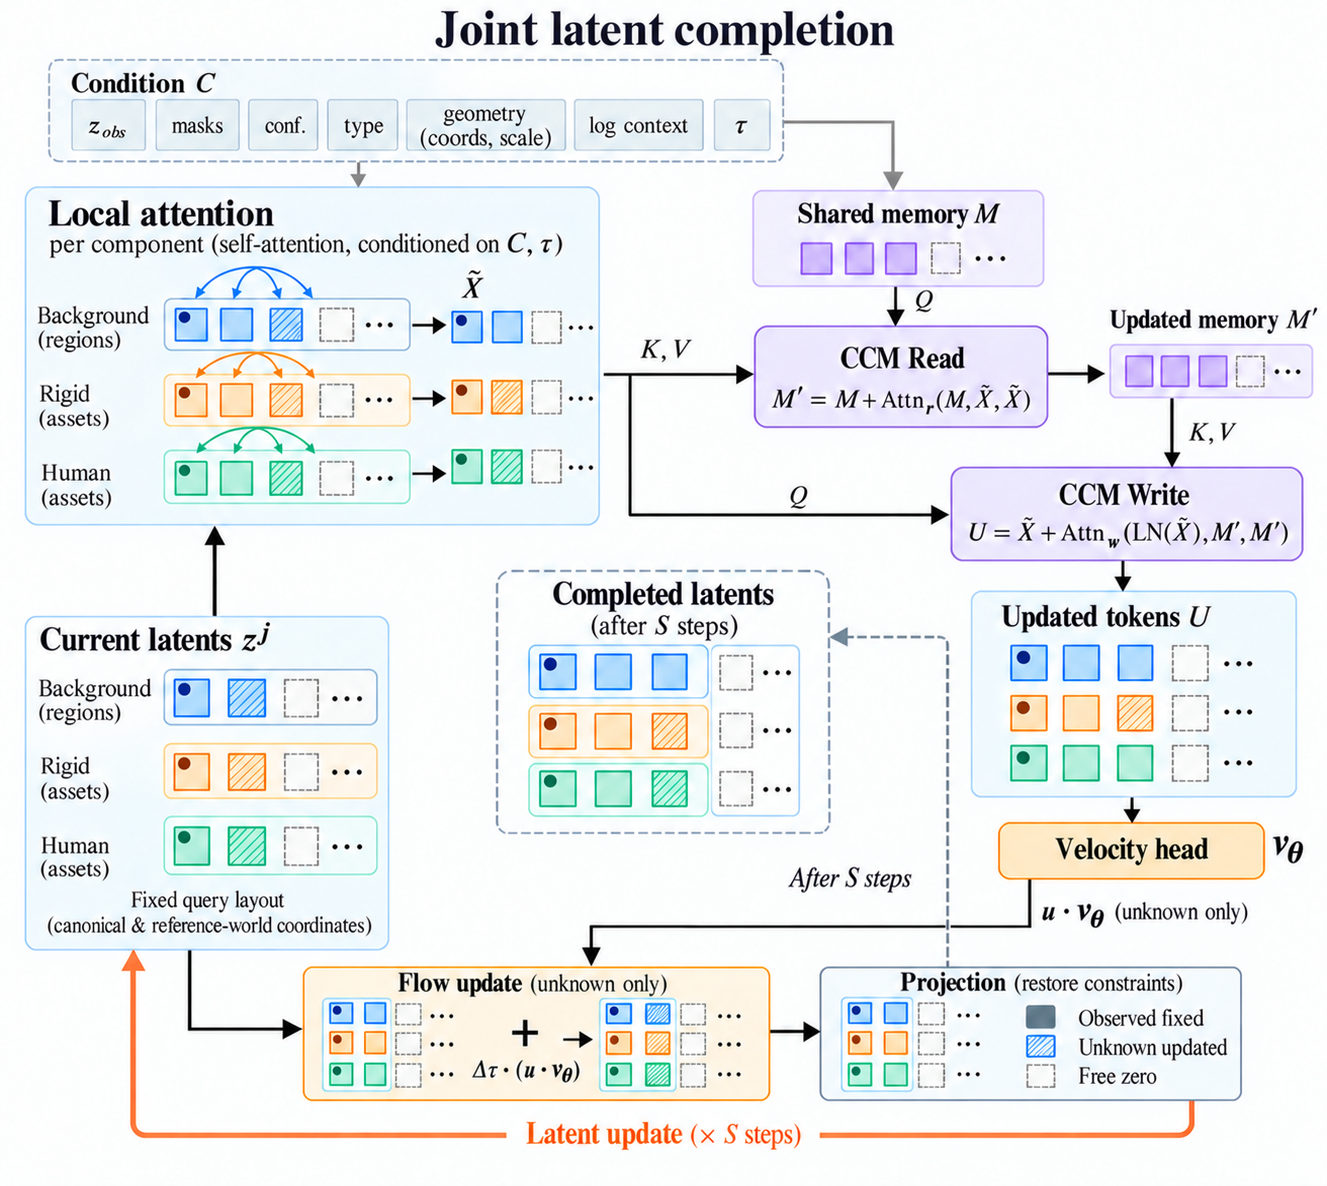
\includegraphics[width=0.86\textwidth]{../fig/drivecompose-joint-completion.png}
\caption{正文联合补全细节图的放大版本。CCM 将组内特征读入共享记忆并写回各组件；速度头与投影更新未知码，同时恢复已见码和清零自由空间码。}
\label{fig:supp-detail}
\end{figure*}
